% introduccion.tex
%
% Describe el objetivo, alcance y contenido del documento.
%
%---------------------------------------------------------

%=========================================================
\chapter{Introducción}

\section{Objetivo del documento}

Objetivo
\noindent El presente documento tiene los siguientes objetivos:\\

\begin{objetivosDoc}
	\item Objetivos
\end{objetivosDoc}

%---------------------------------------------------------
\section{Alcance del documento}

Alcance. \\
\begin{UClist}
	\UCli { Generación de Convocatoria}.
\end{UClist}


%---------------------------------------------------------
\section{Organización del documento}
Organizacion

%---------------------------------------------------------
\section{Diagramas BPMN}

Los diagramas BPMN\footnote{Notación para el Modelado de Procesos de Negocio o BPMN por sus siglas en Inglés (Business Process Modeling Notation).} son una notación gráfica estandarizada que permite el modelado de procesos de negocio en un formato de flujo de trabajo, el objetivo es proporcionar una notación estándar que sea fácilmente legible y entendible por parte de todos los involucrados e interesados del negocio\footnote{Para más información sobre BPMN, revisar los documentos IntroBPMN y DocBPMN.}.\\

\noindent Los diagramas BPMN, a diferencia de los diagramas de flujo, permiten modelar el flujo de información entre diversas áreas y organizaciones, el tiempo que toma realizar cierta tarea y los productos generados. Por lo que se determinó la conveniencia de modelar el proceso de admisión de lass \cdtRef{Actor:EscuelaLibreDeDerecho}{Escuela Libre de Derecho} a través de este estándar.

%\noindent Los diagramas BPMN tienen la característica de mostrar la interacción existente entre las diferentes áreas, entidades o actores de la organización, esto permite visualizar el flujo de la información a través de las áreas.\\

%---------------------------------------------------------
\subsection{Procesos, Subprocesos y Tareas}

{\bf Proceso.} Es una serie de actividades (coordinadas u organizadas) bien definidas, que se realizan (alternativa o simultáneamente) bajo ciertas circunstancias con un fin determinado. Un proceso puede involucrar: ninguno o más de un {\bf subproceso} y una o varias {\bf tareas}.\\
% 	\begin{figure}[!h]
% 	\centering\noindent{
\includegraphics[width=225pt]{images/procesos/bpmn/CollapsedSubprocess.png}}%
% 	\caption{Diagrama de un proceso.}
% 	\label{Intro:CollapsedSubprocess}
% 	\end{figure}

{\bf Subproceso.} Es muy similar al {\bf proceso}, con la única diferencia de que éste sólo puede existir o suceder dentro de un proceso. Está representado por la Figura \ref{Intro:iProceso}.\\
 	\begin{figure}[!h]
 	\centering\noindent{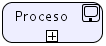
\includegraphics[width=71pt]{images/procesos/SubProceso}}%
 	\caption{Representación de un Proceso y/o Subproceso.}
 	\label{Intro:iProceso}
 	\end{figure}
% 	\begin{figure}[!h]
% 	\centering\noindent{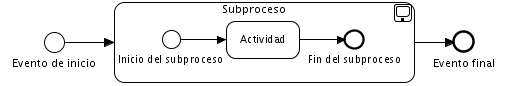
\includegraphics[width=360pt]{images/procesos/bpmn/ExpandedSubprocess.png}}%
% 	\caption{Diagrama de un subproceso expandido.}
% 	\label{Intro:ExpandedSubprocess}
% 	\end{figure}

{\bf Tarea o Actividad.} Es el grado de especificación más simple de un proceso (i.e; es el máximo detalle al que puede llegar un proceso) y de ella no pueden derivar más subprocesos o tareas. Está representado por la Figura \ref{Intro:iTarea}.
 	\begin{figure}[!h]
 	\centering\noindent{
\includegraphics[width=68pt]{images/procesos/Tarea}}%
 	\caption{Representación de una Tarea.}
 	\label{Intro:iTarea}
 	\end{figure}
% 	\begin{figure}[!h]
% 	\centering\noindent{
\includegraphics[width=240pt]{images/procesos/bpmn/SubprocessDiagram.png}}%
% 	\caption{Diagrama de un subproceso colapsado.}
% 	\label{Intro:CollapsedSubprocess}
% 	\end{figure}


%---------------------------------------------------------
\subsection{Subprocesos expandidos y contraídos}

{\bf Subproceso expandido.} Los subprocesos en BPMN, pueden representarse como se muestra en la Figura \ref{Intro:ExpandedSubprocess}. Esto significa que un subproceso puede contener varias actividades o subprocesos ``hijos''.
	\begin{figure}[!h]
	\centering\noindent{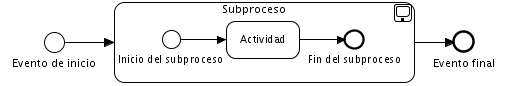
\includegraphics[width=360pt]{images/procesos/bpmn/ExpandedSubprocess.png}}%
	\caption{Subproceso expandido.}
	\label{Intro:ExpandedSubprocess}
	\end{figure}

{\bf Subproceso contraído.} Los subprocesos en BPMN, también pueden representarse como se muestra en la Figura \ref{Intro:CollapsedSubprocess}. Esta representación significa lo mismo que la Figura \ref{Intro:ExpandedSubprocess}, pero sin mostrar explícitamente sus actividades o subprocesos ``hijos''.
	\begin{figure}[!h]
	\centering\noindent{
\includegraphics[width=260pt]{images/procesos/bpmn/CollapsedSubprocess.png}}%
	\caption{Subproceso contraído.}
	\label{Intro:CollapsedSubprocess}
	\end{figure}

% {\bf Diagrama de un subproceso.} Los subprocesos en BPMN, también pueden representarse como en la Figura \ref{Intro:ExpandedCollapsed}. Esta representación significa lo mismo que la Figura \ref{Intro:ExpandedSubprocess}, pero sin mostrar explícitamente sus actividades o subprocesos ``hijos''.
% 	\begin{figure}[!h]
% 	\centering\noindent{
\includegraphics[width=360pt]{images/procesos/bpmn/SubprocessDiagram.png}}%
% 	\caption{Intro:Activity}
% 	\label{Intro:CollapsedSubprocess}
% 	\end{figure}


%---------------------------------------------------------
\subsection{Eventos}

Un {\bf evento} en BPMN representa algo que sucede o podría suceder durante el curso de un proceso y que afecta su flujo. Existen diferentes tipos de eventos:

\begin{itemize}
	\item {\bf Eventos iniciales}. Estos eventos inician el flujo del proceso y no tienen flujos de entrada.

	\arrayrulecolor{white}%
	\begin{tabular}{| m{.08\textwidth} m{.77\textwidth} | }% %{| c{.08\textwidth}  c{.77\textwidth} | }%
		\rowcolor[gray]{0.97}%
		\centering\noindent
\includegraphics[width=18pt]{images/procesos/bpmn/StartEvent.png} & {\bf Evento inicial simple}. No se especifica algún comportamiento en particular para empezar un proceso. \\
		\centering\noindent
\includegraphics[width=18pt]{images/procesos/bpmn/MessageEventStart.png} & {\bf Evento inicial de mensaje}. Un proceso empieza cuando un mensaje es recibido. \\
		\rowcolor[gray]{0.97}%
		\centering\noindent
\includegraphics[width=18pt]{images/procesos/bpmn/TimerEventStart.png} & {\bf Evento inicial de tiempo}. Un proceso empieza en determinada fecha o tiempo específico.
	\end{tabular}%

	\item {\bf Eventos intermedios}. Indican que algo ocurre o podría ocurrir en alguna parte del proceso (desde el inicio y hasta el final). Estos eventos pueden ser usados como parte del flujo de secuencia o adjuntarse a los bordes de una actividad para indicar que la actividad se ejecuta una vez que el evento es activado.

	\arrayrulecolor{white}%
	\begin{tabular}{| m{.08\textwidth} m{.77\textwidth} | }%
		\rowcolor[gray]{0.97}%
		\centering\noindent
\includegraphics[width=18pt]{images/procesos/bpmn/MessageEvent.png} & {\bf Evento intermedio de mensaje}. Indica que un mesaje puede ser enviado o recibido en alguna parte del proceso. \\
		\centering\noindent
\includegraphics[width=18pt]{images/procesos/bpmn/TimerEventIntermediate.png} & {\bf Evento intermedio de tiempo}. Indica que el proceso debe esperar un tiempo especifico para poder continuar.\\
		\rowcolor[gray]{0.97}%
		\centering\noindent
\includegraphics[width=18pt]{images/procesos/bpmn/ConditionalIntermediateEvent.png} & {\bf Evento intermedio de condición}. Se usa cuando el flujo necesita esperar por una condición de negocio para ser completado. Sólo puede usarse dentro de la secuencia del flujo o adjuntado a los bordes de una actividad para indicar que existe un flujo de excepción. \\
		\centering\noindent
\includegraphics[width=18pt]{images/procesos/bpmn/MultipleIntermediateEvent.png} & {\bf Evento intermedio múltiple}. Este evento puede ser activado por muchas causas o sólo por una de ellas. Sólo puede usarse dentro de la secuencia del flujo.\\
		\rowcolor[gray]{0.97}%
		\centering\noindent
\includegraphics[width=18pt]{images/procesos/bpmn/LinkIntermediateEvent.png} & {\bf Evento intermedio de condición}. Este evento permite conectar dos secciones del proceso y puede ser usado únicamente dentro del flujo del proceso.\\
		\centering\noindent
\includegraphics[width=18pt]{images/procesos/bpmn/CompensationIntermediateEvent.png} & {\bf Evento intermedio de compensación}. Permite manejar compensaciones. Puede ser usado dentro de la secuencia del flujo para indicar que se requiere una compensación, o adjuntado a los bordes de una actividad para indicar que la actividad será compensada una vez que el evento sea activado.
	\end{tabular}%

	\item {\bf Eventos finales}. Estos eventos finalizan el flujo del proceso, por lo tanto no pueden tener flujos de salida.

	\arrayrulecolor{white}%
	\begin{tabular}{| m{.08\textwidth} m{.77\textwidth} | }%
		\rowcolor[gray]{0.97}%
		\centering\noindent
\includegraphics[width=18pt]{images/procesos/bpmn/EndEvent.png} & {\bf Evento final.} Indica que el proceso y todas las actividades terminan, sin importar que alguna haya quedado pendiente. \\
		\centering\noindent
\includegraphics[width=18pt]{images/procesos/bpmn/LinkEvent.png} & {\bf Evento final de liga}. Este evento permite conectar dos secciones del proceso. Sólo puede usarse dentro del flujo del proceso.\\
		\centering\noindent
\includegraphics[width=18pt]{images/procesos/bpmn/CancelEndEvent.png} & {\bf Evento final de cancelación}. Permite enviar una excepción de error cuando el flujo llega al final. Este evento solo puede usarse en subprocesos.
	\end{tabular}%
\end{itemize}

%---------------------------------------------------------
\subsection{Compuertas}

Las {\bf compuertas} son elementos usados para controlar la divergencia y convergencia del flujo (separar y unir).\\

	\arrayrulecolor{white}%
	\begin{tabular}{| m{.08\textwidth} m{.77\textwidth} | }%
		\rowcolor[gray]{0.97}%
		\centering\noindent
\includegraphics[width=25pt]{images/procesos/bpmn/ExclusiveGateway.png} & {\bf Compuerta exclusiva basado en los datos}. Como decisión exclusiva, tiene dos o más flujos de secuencia alternos, pero solo uno de ellos puede tomarse basado en la condición de los datos. Como convergencia, es usado para mezclar rutas alternas en una sola. \\
		\centering\noindent
\includegraphics[width=25pt]{images/procesos/bpmn/ParallelGateway.png} & {\bf Compuerta paralela}. Como divergencia, es usada para crear rutas paralelas. Como convergencia, sincroniza multiples rutas paralelas en una. El flujo continúa cuando todas las rutas alcanzan la compuerta. \\
		\rowcolor[gray]{0.97}%
		\centering\noindent
\includegraphics[width=25pt]{images/procesos/bpmn/InclusiveGateway.png} & {\bf Compuerta inclusiva}. Como divergencia, es usada cuando en un punto del flujo una o más rutas puden ser activadas y la decisión está basada en los datos del proceso. Como convergencia, indica que las rutas activas son sincronizadas en una sola.
	\end{tabular}%

%---------------------------------------------------------
\subsection{Conectores}

Los {\bf conectores} son elementos usados para conectar objetos (tareas, subprocesos, eventos, compuertas, etc.) dentro del flujo.\\

	\arrayrulecolor{white}%
	\begin{tabular}{| m{.33\textwidth}  m{.52\textwidth} | }%
		\rowcolor[gray]{0.97}%
		\centering\noindent
\includegraphics[width=120pt]{images/procesos/bpmn/SequenceFlow.png} & {\bf Flujo de secuencia}. Representa el control del flujo y la secuencia de las actividades, compuertas y eventos. \\
		\centering\noindent
\includegraphics[width=120pt]{images/procesos/bpmn/MessageFlow.png} & {\bf Flujo de mensaje}. Es usado para mostrar el flujo de mensajes entre dos entidades o procesos. Representa señales o mensajes, {\bf no el control del flujo}. {\bf No todos los flujos de mensaje son secuenciales o esto especificaría orden en los mensajes}.
	\end{tabular}%


%---------------------------------------------------------
\subsection{Contenedores}

Un {\bf contenedor} es un elemento utilizado en BPMN para distinguir visualmente las responsabilidades entre las áreas u organizaciones.\\

	\arrayrulecolor{white}%
	\begin{tabular}{| m{.33\textwidth}  m{.52\textwidth} | }%
		\rowcolor[gray]{0.97}%
		\centering\noindent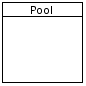
\includegraphics[width=45pt]{images/procesos/bpmn/Pool.png} & {\bf Pool}. Un {\it pool} es un contenedor representando un sólo proceso. \\%El nombre del {\it pool} puede ser considerado el nombre del proceso. \\
		\centering\noindent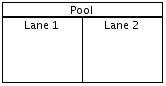
\includegraphics[width=70pt]{images/procesos/bpmn/Lane.png} & {\bf Lane}. Un {\it lane} es una subdivisión de un {\it pool} y representa un rol o área organizacional.
	\end{tabular}%

%---------------------------------------------------------
\subsection{Tipos de subprocesos}

%El {\bf proceso RENIECYT} describe una parte de la funcionalidad del registro RENIECYT, por medio de una serie de actividades bien definidas, con el objetivo de realizar el registro de los usuarios en RENIECYT.\\

Se han dividido los procesos de la \cdtRef{Actor:EscuelaLibreDeDerecho}{Escuela Libre de Derecho} en diversos subprocesos con la finalidad de entender y visualizar mejor su funcionalidad. Estos subprocesos se han clasificado en dos tipos:
\begin{itemize}
	\item Críticos. Son aquellos subprocesos complejos que pueden involucrar más de un subproceso y/o tareas y describen una parte sumamente importante del proceso propuesto para la \cdtRef{Actor:EscuelaLibreDeDerecho}{Escuela Libre de Derecho}. Están representados por la Figura \ref{Intro:iProcesoComplejo}.
	\begin{figure}[!h]
	\centering\noindent{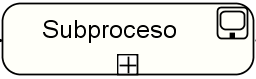
\includegraphics[width=71pt]{images/procesos/SubProcesoComplejo}}%
	\caption{Representación de un Subproceso Complejo.}
	\label{Intro:iProcesoComplejo}
	\end{figure}

	\item Simples. Son subprocesos sencillos y probablemente requieran únicamente de tareas para describir sus actividades. Están representados por la Figura \ref{Intro:iProceso}.
\end{itemize}

\noindent Notese que la única diferencia entre ambos es el color de relleno, los subprocesos críticos son de color amarillo, mientras que los subprocesos simples son de color azul.\\

%\noindent El proceso RENIECYT puede llevar a cabo diversas actividades las cuales pueden ser subprocesos o tareas. Se usa la Figura \ref{Intro:iProcesoComplejo} para indicar que una actividad es un subproceso crítico, la Figura \ref{Intro:iProceso} para indicar que una actividad es un subproceso simple y la Figura \ref{Intro:iTarea} para indicar que una actividad es una tarea.


%---------------------------------------------------------
\subsection{Nombre de los subprocesos}

\noindent Se usa la siguiente estructura para nombrar los subprocesos de Admisión de la \cdtRef{Actor:EscuelaLibreDeDerecho}{Escuela Libre de Derecho}:
	\begin{center}
		{\bf PP- + Tipo de Proceso + Número consecutivo + Nombre del subproceso}
	\end{center}

\noindent Donde:
\begin{itemize}
	\item{\bf PP-}. Significa que es un subproceso propuesto.
	\item{\bf Tipo de Proceso}. Puede tomar uno de los siguientes valores:
		\begin{itemize}
			\item{\bf A}. Significa que es un subproceso de Admisión.
		\end{itemize}
	\item{\bf Número consecutivo}. Estará dado por el nivel de profundidad que presente dicho subproceso. Por ejemplo, en la Figura \ref{Intro:JerarquiaProcesos} el Proceso General tiene un subproceso 1 y un subproceso 2.
		\begin{figure}[!h]
		\centering\noindent{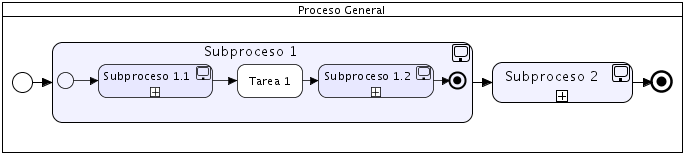
\includegraphics[width=0.87\textwidth]{images/procesos/JerarquiaProcesos_1}}%
		\caption{Subproceso General.}
		\label{Intro:JerarquiaProcesos}
		\end{figure}

		Se puede ver que el subproceso 1 tiene un subproceso 1.1, una tarea 1 y un subproceso 1.2. Si profundizáramos aún más dentro del subproceso 1.1 se verá que realiza dos actividades: tarea 1 y tarea 2, como se muestra en la Figura \ref{Intro:JerarquiaProcesos2}
		\begin{figure}[!h]
		\centering\noindent{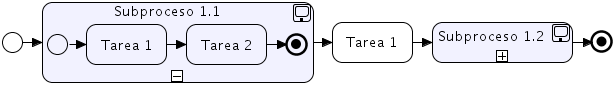
\includegraphics[width=0.8\textwidth]{images/procesos/JerarquiaProcesos2_1}}%
		\caption{Subproceso 1.1.}
		\label{Intro:JerarquiaProcesos2}
		\end{figure}

	\item{\bf Nombre del proceso}. Estará dado por el nombre que presente el subproceso o actividad en el diagrama BPMN.
\end{itemize}

\noindent Por ejemplo:
	\begin{center}
		{\bf PP-A 1.5.1 Pago SPEI}
	\end{center}

\noindent Significa que es el subproceso \textbf{PP-} de Admisión \textbf{A} número \textbf{5} que contiene el subroceso \textbf{1} llamado \textbf{Pago SPEI}.

%---------------------------------------------------------
\subsection{Elementos de un subproceso}

Un {\bf elemento} del subproceso es un atributo utilizado para describir las características de los subprocesos. Los atributos ayudan a entender la funcionalidad e interacción de un subproceso con otro (a través de los insumos de entrada y productos de salida).\\

\noindent Los elementos que describen los subprocesos de Admisión son los siguientes:

\begin{itemize}
	\item {\bf Actores:} Lista de los actores que intervienen en el subproceso.
	\item {\bf Objetivo:} Breve descripción del propósito del subproceso.
	\item {\bf Insumos de entrada:} Lista de datos de entrada requeridos durante la ejecución del subproceso.
	\item {\bf Proveedores:} Son las áreas o personas que proveen insumos al subproceso.
	\item {\bf Productos de salida:} Lista de datos de salida que otorga el subproceso al ser ejecutado.
	\item {\bf Cliente:} Áreas o personas que consumen los productos generados por el subproceso.
	\item {\bf Recursos del proceso}: Son los recursos necesarios para llevar a cabo el subproceso.
	\item {\bf Interrelación con otros procesos:} Es la interacción con otros subprocesos internos y/o externos para verificar la apropiada interacción con estos.
\end{itemize}
